\chapter{Complex Numbers}

\section{Definition and arithmetic}

\begin{definition}
A \emph{complex number} is an expression $z = x + yi$ with $x, y \in \R$, where $i^2 = -1$.
$x = \RE(z)$ is the \emph{real part} and $y = \IM(z)$ the \emph{imaginary part} (a real number).
The set of complex numbers is $\C$. Two complex numbers are equal iff their real parts are equal
and their imaginary parts are equal.
\end{definition}

Arithmetic follows the usual rules with $i^2 = -1$:
\begin{align*}
(a + bi) + (c + di) &= (a+c) + (b+d)i,\\
(a + bi)(c + di) &= (ac - bd) + (ad + bc)i.
\end{align*}
Powers of $i$ cycle with period $4$: $i, -1, -i, 1, i, \dots$; e.g.\ $i^{103} = i^{100}i^3 = -i$.

\begin{example}
$(3 + 2i)(1 - 4i) = 3 - 12i + 2i - 8i^2 = 3 + 8 - 10i = 11 - 10i$.
\end{example}

\begin{proposition}
Every non-zero $z = x + yi$ has a multiplicative inverse
$z^{-1} = \dfrac{x - yi}{x^2 + y^2}$. With the operations above, $\C$ is a field.
\end{proposition}

\section{Conjugate and modulus}

\begin{definition}
The \emph{conjugate} of $z = x + yi$ is $\conj z = x - yi$. The \emph{modulus} is
$\abs z = \sqrt{x^2 + y^2}$, a non-negative real number.
\end{definition}

\begin{proposition}[Properties of Conjugate, PCJ]
For $z,w \in \C$:
\begin{enumerate}
  \item $\conj{\conj z} = z$, $\conj{z + w} = \conj z + \conj w$, $\conj{zw} = \conj z\,\conj w$,
        $\conj{z/w} = \conj z/\conj w$ ($w\neq0$);
  \item $z + \conj z = 2\RE(z)$ and $z - \conj z = 2i\IM(z)$;
  \item $z \in \R \iff z = \conj z$, and $z$ is purely imaginary iff $\conj z = -z$;
  \item $z\conj z = \abs z^2$.
\end{enumerate}
\end{proposition}

\begin{proposition}[Properties of Modulus, PM]
\begin{enumerate}
  \item $\abs z = 0 \iff z = 0$; $\abs{\conj z} = \abs z$;
  \item $\abs{zw} = \abs z\abs w$ and $\abs{z/w} = \abs z/\abs w$;
  \item (Triangle inequality) $\abs{z + w} \le \abs z + \abs w$.
\end{enumerate}
\end{proposition}
\begin{proof}[Proof of the triangle inequality]
$\abs{z+w}^2 = (z+w)(\conj z + \conj w) = \abs z^2 + z\conj w + \conj{z\conj w} + \abs w^2
= \abs z^2 + 2\RE(z\conj w) + \abs w^2 \le \abs z^2 + 2\abs{z}\abs{w} + \abs w^2 =
(\abs z + \abs w)^2$, using $\RE(u) \le \abs u$. Take square roots.
\end{proof}

Division is done by multiplying numerator and denominator by the conjugate of the denominator.

\begin{example}
$\dfrac{2 + 3i}{1 - i} = \dfrac{(2+3i)(1+i)}{(1-i)(1+i)} = \dfrac{2 + 2i + 3i + 3i^2}{2}
= \dfrac{-1 + 5i}{2} = -\dfrac12 + \dfrac52 i$.
\end{example}

\begin{example}[Square roots algebraically]
Solve $z^2 = -3 + 4i$. Write $z = a + bi$: $a^2 - b^2 = -3$ and $2ab = 4$. Also
$\abs z^2 = \abs{-3+4i} = 5$, so $a^2 + b^2 = 5$. Adding, $a^2 = 1$; subtracting, $b^2 = 4$. Since
$ab = 2 > 0$, $a,b$ have the same sign: $z = \pm(1 + 2i)$. Check: $(1+2i)^2 = 1 + 4i - 4 = -3+4i$.
\end{example}

\begin{example}[Complex quadratic]
Solve $z^2 + 2z + (1 - 2i) = 0$. The quadratic formula holds over $\C$:
discriminant $\Delta = 4 - 4(1 - 2i) = 8i$. A square root of $8i$ is $2 + 2i$ since
$(2+2i)^2 = 4 + 8i - 4 = 8i$. So $z = \frac{-2 \pm (2 + 2i)}{2}$, i.e.\ $z = i$ or $z = -2 - i$.
Check: $i^2 + 2i + 1 - 2i = 0$.
\end{example}

\section{The complex plane and polar form}

Identify $z = x + yi$ with the point $(x,y)$ in the \emph{complex plane} (Argand diagram):
the horizontal axis is the real axis and the vertical axis the imaginary axis. $\abs z$ is the
distance from $0$, $\conj z$ is the reflection in the real axis, and addition is vector
addition.

\begin{center}
\begin{tikzpicture}[scale=1.1]
  \draw[->] (-0.5,0) -- (3,0) node[right] {$\RE$};
  \draw[->] (0,-1.8) -- (0,2.2) node[above] {$\IM$};
  \draw[thick,->] (0,0) -- (2.2,1.5) node[above right] {$z = x + yi$};
  \draw[dashed] (2.2,1.5) -- (2.2,0) node[below] {$x$};
  \draw[dashed] (2.2,1.5) -- (0,1.5) node[left] {$y$};
  \draw[->] (0,0) -- (2.2,-1.5) node[below right] {$\conj z$};
  \draw (0.7,0) arc (0:34:0.7);
  \node at (0.95,0.25) {$\theta$};
  \node at (0.9,0.95) {$r$};
\end{tikzpicture}
\end{center}

\begin{definition}
If $z \ne 0$ has modulus $r = \abs z$ and makes angle $\theta$ with the positive real axis,
then
\[ z = r(\cos\theta + i\sin\theta), \]
the \emph{polar form} of $z$. Any such $\theta$ is an \emph{argument} of $z$; arguments are
determined up to multiples of $2\pi$. We abbreviate $\cos\theta + i\sin\theta = \cis\theta$
and also write it $e^{i\theta}$.
\end{definition}

To convert: $r = \sqrt{x^2+y^2}$, and $\theta$ satisfies $\cos\theta = x/r$, $\sin\theta = y/r$
(choose the quadrant from the signs of $x$ and $y$; $\tan\theta = y/x$ alone is ambiguous).

\begin{example}
$1 + i\sqrt3$: $r = 2$, $\cos\theta = \frac12$, $\sin\theta = \frac{\sqrt3}2$, so
$\theta = \frac\pi3$ and $1 + i\sqrt 3 = 2\cis\frac\pi3$.
$-1 - i$: $r = \sqrt2$, third quadrant, $\theta = \frac{5\pi}{4}$, so $-1 - i = \sqrt2\cis\frac{5\pi}4$.
\end{example}

\begin{theorem}[Polar Multiplication]
$r_1\cis\theta_1\cdot r_2\cis\theta_2 = r_1r_2\cis(\theta_1 + \theta_2)$.
\end{theorem}
\begin{proof}
Expand and use the angle-sum identities:
$(\cos\theta_1 + i\sin\theta_1)(\cos\theta_2 + i\sin\theta_2) = (\cos\theta_1\cos\theta_2 -
\sin\theta_1\sin\theta_2) + i(\sin\theta_1\cos\theta_2 + \cos\theta_1\sin\theta_2) =
\cos(\theta_1+\theta_2) + i\sin(\theta_1 + \theta_2)$.
\end{proof}

So multiplying complex numbers multiplies moduli and \emph{adds} arguments; multiplying by
$i = \cis\frac\pi2$ rotates by $90^\circ$.

For example, $(1+i)(1 + i\sqrt3) = \sqrt2\cis\frac\pi4 \cdot 2\cis\frac\pi3
= 2\sqrt2\cis\frac{7\pi}{12}$:
\begin{center}
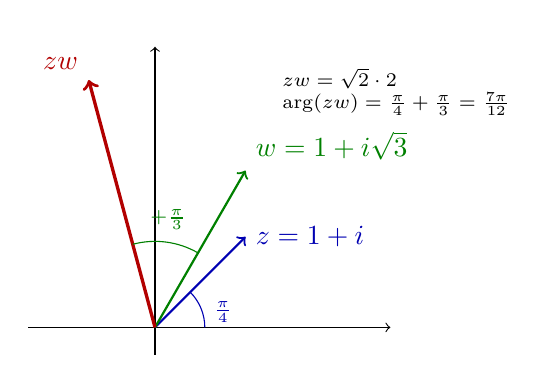
\begin{tikzpicture}[scale=1.15]
  \draw[->] (-1.4,0) -- (2.6,0) node[right] {$\RE$};
  \draw[->] (0,-0.3) -- (0,3.1) node[above] {$\IM$};
  \draw[thick,->,blue!70!black] (0,0) -- (1,1) node[right] {$z = 1 + i$};
  \draw[thick,->,green!50!black] (0,0) -- (1,1.732) node[above right] {$w = 1 + i\sqrt3$};
  \draw[very thick,->,red!70!black] (0,0) -- ({2.828*cos(105)},{2.828*sin(105)}) node[above left] {$zw$};
  \draw[blue!70!black] (0.55,0) arc (0:45:0.55); \node[blue!70!black,font=\scriptsize] at (0.75,0.17) {$\frac\pi4$};
  \draw[green!50!black] (60:0.95) arc (60:105:0.95);
  \node[green!50!black,font=\scriptsize] at (83:1.2) {$+\frac\pi3$};
  \node[font=\scriptsize,align=left,right] at (1.3,2.6) {$\abs{zw} = \sqrt2 \cdot 2$\\$\arg(zw) = \frac\pi4 + \frac\pi3 = \frac{7\pi}{12}$};
\end{tikzpicture}
\end{center}

\section{De Moivre's theorem}

\begin{theorem}[De Moivre's Theorem, DMT]
For all $\theta \in \R$ and $n \in \Z$, $(\cos\theta + i\sin\theta)^n = \cos(n\theta) +
i\sin(n\theta)$.
\end{theorem}
\begin{proof}
For $n \ge 0$, induction: $n = 0$ gives $1 = 1$, and $(\cis\theta)^{k+1} = \cis(k\theta)\cis\theta
= \cis((k+1)\theta)$ by polar multiplication. For $n = -m < 0$:
$(\cis\theta)^{-m} = 1/\cis(m\theta) = \cis(-m\theta)$, since $\cis(m\theta)\cis(-m\theta) =
\cis 0 = 1$.
\end{proof}

\begin{example}
Compute $(1 + i\sqrt3)^{10}$:
\[ (2\cis\tfrac\pi3)^{10} = 2^{10}\cis\tfrac{10\pi}{3} = 1024\cis\tfrac{4\pi}{3}
= 1024\left(-\tfrac12 - \tfrac{\sqrt3}2 i\right) = -512 - 512\sqrt3\, i. \]
\end{example}

\begin{example}
$(1 - i)^{8} = (\sqrt 2\cis(-\tfrac\pi4))^8 = 16\cis(-2\pi) = 16$.
\end{example}

\begin{example}[Trig identities]
By DMT and the binomial theorem, $\cos3\theta + i\sin 3\theta = (c + is)^3 = c^3 + 3ic^2s - 3cs^2
- is^3$ where $c = \cos\theta$, $s = \sin\theta$. Comparing real parts,
$\cos3\theta = c^3 - 3cs^2 = c^3 - 3c(1 - c^2) = 4\cos^3\theta - 3\cos\theta$.
\end{example}

\section{The complex exponential}

\begin{definition}
For $\theta\in\R$ define $e^{i\theta} = \cos\theta + i\sin\theta$ (Euler's formula). For
$z = x + yi$, $e^{z} = e^x e^{iy}$.
\end{definition}

With this notation polar multiplication is $e^{i\theta_1}e^{i\theta_2} = e^{i(\theta_1+\theta_2)}$
and DMT reads $(e^{i\theta})^n = e^{in\theta}$, just like real exponent laws. Every non-zero
$z$ can be written $z = re^{i\theta}$. Famous special case: $e^{i\pi} + 1 = 0$. Also
$\conj{e^{i\theta}} = e^{-i\theta}$, so $\cos\theta = \frac{e^{i\theta} + e^{-i\theta}}2$.

\section{n-th roots}

\begin{theorem}[Complex $n$-th Roots Theorem, CNRT]
Let $a = r\cis\theta \neq 0$ and $n \in \N$. The equation $z^n = a$ has exactly $n$ distinct
solutions
\[ z_k = \sqrt[n]{r}\,\cis\left(\frac{\theta + 2\pi k}{n}\right), \qquad k = 0,1,\dots,n-1, \]
where $\sqrt[n] r$ is the positive real $n$-th root.
\end{theorem}
\begin{proof}
Write $z = s\cis\varphi$. By DMT, $z^n = s^n\cis(n\varphi) = r\cis\theta$ iff $s^n = r$ and
$n\varphi = \theta + 2\pi k$ for some integer $k$. So $s = \sqrt[n]r$ and
$\varphi = \frac{\theta + 2\pi k}{n}$. Values of $k$ that are congruent mod $n$ give the same
angle up to a multiple of $2\pi$, and $k = 0,\dots,n-1$ give $n$ angles in $[\frac\theta n,
\frac\theta n + 2\pi)$, which are distinct points.
\end{proof}

The $n$-th roots lie on a circle of radius $\sqrt[n]r$, equally spaced at angles $2\pi/n$: the
vertices of a regular $n$-gon.

\begin{example}
Solve $z^3 = 8i$. $8i = 8\cis\frac\pi2$, so $z_k = 2\cis\left(\frac\pi6 + \frac{2\pi k}{3}\right)$:
\begin{align*}
z_0 &= 2\cis\tfrac\pi6 = \sqrt3 + i,\\
z_1 &= 2\cis\tfrac{5\pi}6 = -\sqrt3 + i,\\
z_2 &= 2\cis\tfrac{3\pi}2 = -2i.
\end{align*}
Check: $(-2i)^3 = -8i^3 = 8i$.
\end{example}

\begin{center}
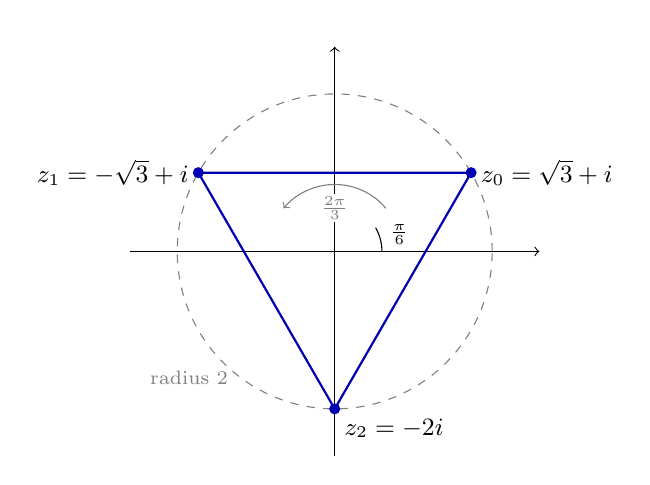
\begin{tikzpicture}[scale=1.0]
  \draw[->] (-2.6,0) -- (2.6,0) node[right] {$\RE$};
  \draw[->] (0,-2.6) -- (0,2.6) node[above] {$\IM$};
  \draw[gray,dashed] (0,0) circle (2);
  \draw[blue!70!black,thick] (30:2) -- (150:2) -- (270:2) -- cycle;
  \foreach \a/\lab/\pos in {30/{z_0 = \sqrt3 + i}/right, 150/{z_1 = -\sqrt3 + i}/left, 270/{z_2 = -2i}/below right} {
    \fill[blue!70!black] (\a:2) circle (2pt);
    \node[\pos,font=\small] at (\a:2) {$\lab$};
  }
  \draw (0.6,0) arc (0:30:0.6); \node[font=\scriptsize] at (15:0.85) {$\frac\pi6$};
  \draw[->,gray] (40:0.85) arc (40:140:0.85); \node[gray,font=\scriptsize,fill=white,inner sep=1pt] at (90:0.55) {$\frac{2\pi}3$};
  \node[font=\scriptsize,gray] at (-1.85,-1.6) {radius $2$};
\end{tikzpicture}
\end{center}
The three cube roots of $8i$ form an equilateral triangle on the circle of radius
$\sqrt[3]8 = 2$, starting at angle $\frac\pi6 = \frac13\cdot\frac\pi2$.

\begin{example}
Solve $z^4 = -16$. $-16 = 16\cis\pi$, so $z_k = 2\cis\frac{\pi + 2\pi k}{4}$, $k = 0,1,2,3$:
$\pm\sqrt2 \pm\sqrt2 i$ (all four sign combinations).
\end{example}

\section{Roots of unity}

\begin{definition}
The solutions of $z^n = 1$ are the \emph{$n$-th roots of unity}:
$\omega_k = \cis\frac{2\pi k}{n} = e^{2\pi i k/n}$, $k = 0,\dots,n-1$. With
$\omega = \omega_1$, they are $1, \omega, \omega^2, \dots,\omega^{n-1}$.
\end{definition}

\begin{example}
Cube roots of unity: $1$, $\omega = -\frac12 + \frac{\sqrt3}2 i$, $\omega^2 = -\frac12 -
\frac{\sqrt3}2 i$. Since $z^3 - 1 = (z-1)(z^2 + z + 1)$, we get $1 + \omega + \omega^2 = 0$.
Sixth roots of unity: $\pm1$, $\pm\frac12\pm\frac{\sqrt3}2 i$.
\end{example}

\begin{center}
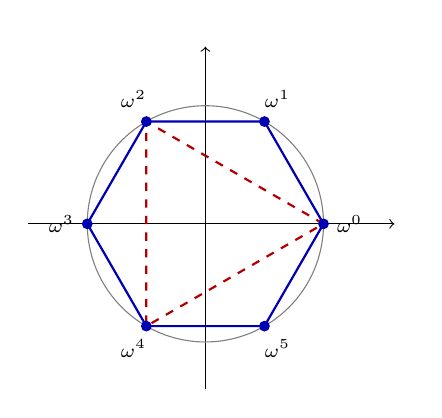
\begin{tikzpicture}[scale=1.5]
  \draw[->] (-1.5,0) -- (1.6,0) node[right] {$\RE$};
  \draw[->] (0,-1.4) -- (0,1.5) node[above] {$\IM$};
  \draw[gray] (0,0) circle (1);
  \draw[blue!70!black,thick] (0:1) -- (60:1) -- (120:1) -- (180:1) -- (240:1) -- (300:1) -- cycle;
  \draw[red!70!black,thick,dashed] (0:1) -- (120:1) -- (240:1) -- cycle;
  \foreach \k in {0,...,5} {
    \fill[blue!70!black] ({60*\k}:1) circle (1.3pt);
    \node[font=\scriptsize] at ({60*\k}:1.22) {$\omega^{\k}$};
  }
\end{tikzpicture}
\end{center}
The sixth roots of unity $\omega^k$ ($\omega = \cis\frac\pi3$) form a regular hexagon; every
second one ($1, \omega^2, \omega^4$, dashed) is a cube root of unity. The vertices are
symmetric about $0$, which is one way to see that they sum to $0$.

\begin{proposition}
For $n \ge 2$, the $n$-th roots of unity sum to $0$: $\sum_{k=0}^{n-1}\omega^k =
\frac{\omega^n - 1}{\omega - 1} = 0$. If $z^n = a$ has a solution $z_0$, then all solutions are
$z_0\omega^k$.
\end{proposition}

\section{Common pitfalls}
\begin{itemize}
  \item Calling $bi$ the imaginary part; $\IM(a + bi) = b$, a real number.
  \item Choosing the wrong quadrant for the argument from $\arctan(y/x)$.
  \item Giving only one $n$-th root, or listing $n+1$ of them (the $k = n$ root repeats $k=0$).
  \item Writing $\sqrt{z}$ for complex $z$ as though it were a single well-defined value.
  \item $\abs{z + w} \ne \abs z + \abs w$ in general.
\end{itemize}

\section{Summary}
\begin{itemize}
  \item $\C$ is a field; divide by multiplying by the conjugate; $z\conj z = \abs z^2$.
  \item Polar form $z = r\cis\theta = re^{i\theta}$; multiplication multiplies moduli and adds
        arguments.
  \item DMT: $(\cis\theta)^n = \cis(n\theta)$, for computing powers and deriving identities.
  \item CNRT: $z^n = r\cis\theta$ has $n$ roots $\sqrt[n]r\cis\frac{\theta + 2\pi k}{n}$; the
        $n$-th roots of unity are $e^{2\pi ik/n}$ and sum to $0$.
\end{itemize}
